% ------------------------------------------------------------------
            \subsubsection{Dyslextia}
            
                \paragraph{Dyslextia: Struggles}\\
                \begin{itemize}
                    \item \textbf{Leesvaardigheden}\cite{dyslextia-struggles-and-superpowers}:
                        Dit is waaschijnlijk de meest bekende problemen die mensen met Dyslextia hebben. 

                    \item \textbf{Schrijfvaardigheden}:
                        Dit is waaschijnlijk het andere meest bekende probleem die mensen met Dyslextia hebben.
                        
                    \item \textbf{Het omkeren van letters en cijfers tijdens het lezen (bijvoorbeeld "zag" lezen als "was")}\cite{dyslextia-struggles-and-superpowers}:
                        Een veel voorkomend probleem is het omkeren van letters zoals 'b' en 'd', of 'p' en 'q'. Gezien dit de zelfde letter is maar dan geroteerd, of gespiegeld.
                        
                    \item \textbf{Notities maken in lessen en lezingen}\cite{dyslextia-struggles-and-superpowers}:
                        Gezien het Lezen en Schrijfven al lastig is, is het voor dyslexten bijna onmogelijk om zowel te lezen, schrijven en luisteren te gelijker tijd.
                    
                    \item \textbf{Sequentiële instructies volgen}\cite{dyslextia-struggles-and-superpowers}:
                        Dit heeft wederom te maken met werk geheugen. Mensen met dyslextie hebben er niet perse minder van zoals met ADHD. Maar het is gebleken dat er verschillende soorten werkgeheugen zijn\cite{dyslextia-different-types-of-memory}. Voornamelijk visueel en auditorisch. (theoretisch zijn er meer vormen. Voor elk zintuig een). Om dingen het beste te onthouden moet men zo veel mogelijk van deze te gelijker tijd gebruiken. Dit geeft je de grootste kans iets te herinneren. Hier is het probleem, mensen met dyslextie hebben een dramatisch slechter auditorisch geheugen. Wat dus betekend dat je daar minder op kan leunen, en daarom alleen maar visueel informatie kan op slaan. Dat betekend dan dus dat je als dyslext minder goed dingen kan onthouden. Je kan namelijk maar gebuik maken van een van de twee smaken.
                        
                    \item \textbf{Woorden, zinnen en namen onthouden}\cite{dyslextia-struggles-and-superpowers}:
                        Mensen onthouden woorden, zinnen, en namen voornamelijk auditorisch. Je onthoud het geheugen van hoe het woord, de zin, of die naam ook al weer klonk. Niet hoe je het ookal weer spelde, of hoe het woord er uit zag. Dit maakt dus dat je als dyslext deze dingen minder goed kan onthouden. Zoals uitgelegd in het punt hierboven.
                        
                    \item \textbf{Geschreven lijsten en telefoonnummers memoriseren}\cite{dyslextia-struggles-and-superpowers}:
                        
                    
                    \item \textbf{Woordrekenproblemen begrijpen}\cite{dyslextia-struggles-and-superpowers}:
                        Het probleem hiermee is omdat dyslexten zoals hierboven auditorisch niet goed dingen kunnen onthouden. Het onthouden van dit verhaal waarin zich een reken probleem voorkomt het moeilijker is om deze informatie er uit te halen. Dat heeft niks te maken met dat ze minder goed kunen rekenen, maar het process om deze informatie uit te vissen is gewoon moeilijker voor ons.
                        
                    \item \textbf{Hun ideeën op georganiseerde wijze uitdrukken}\cite{dyslextia-struggles-and-superpowers}:
                        ik wil mijn punt over werk geheugen niet blijven herhalen, maar ik denk dat ik dat nog een keer moet
                        
                \end{itemize}
                
                % — — — — — — — — — — — — — — — — — — — — — — — — — — — — — — — 
                \bigskip
                \noindent\paragraph{Dyslextia: Sterktes}\\
                \begin{itemize}
                    \item \textbf{Seeing the big picture}\cite{dyslextia-struggles-and-superpowers}:
                        Dyslexten zijn beter in de bigger picture zien dan hun neurotypische teggeliggers.
                        
                    \item \textbf{Het vinden van complexen patronen en verstoring}\cite{dyslextia-struggles-and-superpowers}:
                        Vergelijkbaar met het een van de sterkste voordelen van autisme hebben dislexten een voordeel dat ze veel sneller en veel beter complexen patronen, en verstoring in dat patroon kunnen vinden.
                        
                    \item \textbf{Ruimtelijk inzicht en manipulatie}\cite{dyslextia-struggles-and-superpowers}:
                        Dyslexten zijn net zoals de meeste neurodivergente mensen visueel ingesteld. Ze zijn hier ook een stuk beter in dan neurotypicals. Omdat ze niet 
                        
                    \item \textbf{Visual thinking}\cite{dyslextia-struggles-and-superpowers}:
                        Mensen met dyslextie hebben een veel beter ruimtelijk inzicht en denk vermogen. Is dit waarom de letter op het papier bewegen en draaien? Geen idee.
                        
                    \item {\textbf{Thinking outside the box}\cite{dyslextia-struggles-and-superpowers}:
                        hier volgt een letterlijke vertaling van bron \cite{Creativity-and-Dyslexia} over waarom dyslexten creativer zijn:
                        {"\textit{De meeste mensen met dyslexie hebben de neiging om in beelden te denken in plaats van in woorden, dit komt deels door de activatie van delen van de hersenen" (Jones, 2016) die de meeste volwassenen vaak niet gebruiken. Als gevolg daarvan is wat anderen als innovatief of creatief beschouwen voor een dyslecticus vanzelfsprekend.}"}
                        }
                \end{itemize}

                    
                % — — — — — — — — — — — — — — — — — — — — — — — — — — — — — — — 
                \bigskip
                \noindent\textbf{Dyslextia: Les tips}
                    \begin{itemize}
                        \item{\textbf{Gebruik \hyperlink{https://opendyslexic.org/}{OpenDyslextic}}. 
                            Dit is een lettertype speciaal gemaakt voor mensen met dyslextie. Sterker nog. Ik wou alles in dit lettertype schrijven, dit hele document. Alleen hier heb ik 2 uur op verloren omdat ik maar problemen bleef hebben met \LaTeX. Trust me, I really tried. Dat is ook de rede dat dit document niet zwart op wit is. Ik heb geprobeerd het zo dyslextie vriendelijk te maken. 
                            
                            \bigskip
                            
                            \begin{center}
                                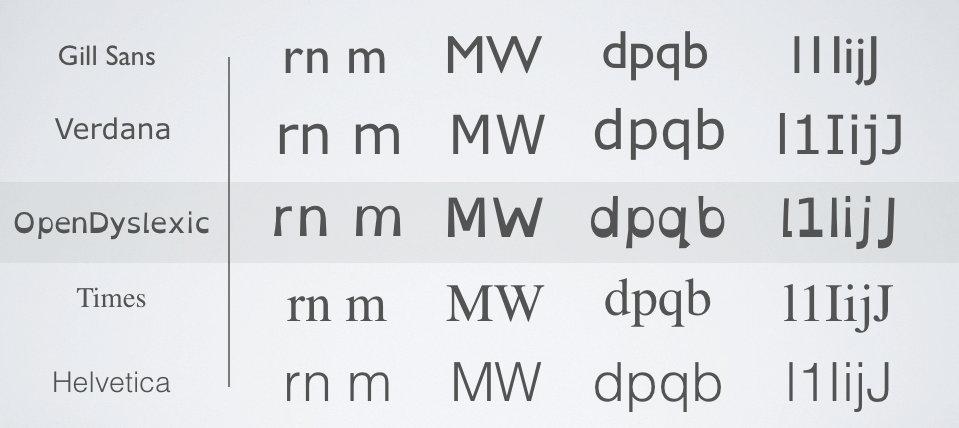
\includegraphics[width=35em]{Eindopdracht-Tygo-van-den-Hurk-1705709/Resources/Images/open-dyslexic-abelardo-gonzalez-font-character-map.png}
                            \end{center}
                            
                            \bigskip
                            
                            \noindent Het is misschien een lelijk lettertype. — Althans dat vond ik in het begin. — Maar heb dit lettertype gebuikt de afgelopen maand het het leest veel fijner naar mijn mening. De eerste paar dagen moest ik echt wennen. Ik moest een soort van op nieuw leren lezen. Maar nu? Nu is het veel veel fijner. Ik gebruik extensies om dit lettertype te forceren. Dit is bijna het enige lettertype dat ik lees.
                            
                            \bigskip
                            
                            \noindent Een probleem dat veel mensen met dyslextie hebben is dat letters draaien en verplaatsen als je ze leest. Zoals je het in de film ziet. — though niet altijd even erg. — Als ik OpenDyslextic gebruik heb ik dit probleem niet meer. Ze blijven gewoon stil staan. Dat niet alleen, Letters lijken ook minder op elkaar.
                            
                            \bigskip
                            
                            \noindent Ik kan niet de enige zijn die ooit heeft opgemerkt dat van deze zes letters: \texttt{p}, \texttt{q}, \texttt{b}, \texttt{d}, \texttt{O}, \texttt{0}; het er maar twee zijn. \texttt{d} \& \texttt{O} zijn allemaal het zelfde. En dat is echt heel irritant. Zeker als je even een mindere dag hebt waar de letters op je papiertje net soep zijn. Kijk OpenDyslexic kan geen wonderen maken, maar kijk naar de afbeelding, ze hebben ze verschillend gemaakt. Dit maakt ze zo veel minder vermoeiend om te lezen.
                            
                            \bigskip
                            
                            \noindent Ze hebben ook funky dingen gedaan met de spacing van de letters etc. Ik kan hier uren over door gaan. Punt is, dit is een upgrade, gebruik het. Als je meer wil weten, of dit lettertype \textbf{gratis} wil downloaden, ga dan naar \underline{\hyperlink{https://opendyslexic.org/}{opendyslexic.org}.
                        }

                        \item{\textbf{Houd het visueel}. 
                            Net zoals bij de tips voor ADHD, en autisme is het belangrijk dat je dingen visueel houd. Zeker gezien lezen vaak een probleem is. Plaatjes, grafieken, en diagramen zijn een god sent.
                        }
                    \end{itemize}
